\usetikzlibrary{shapes.geometric};
\usetikzlibrary{fit};
\pgfdeclarelayer{background}
\pgfdeclarelayer{foreground}
\pgfsetlayers{background,main,foreground}
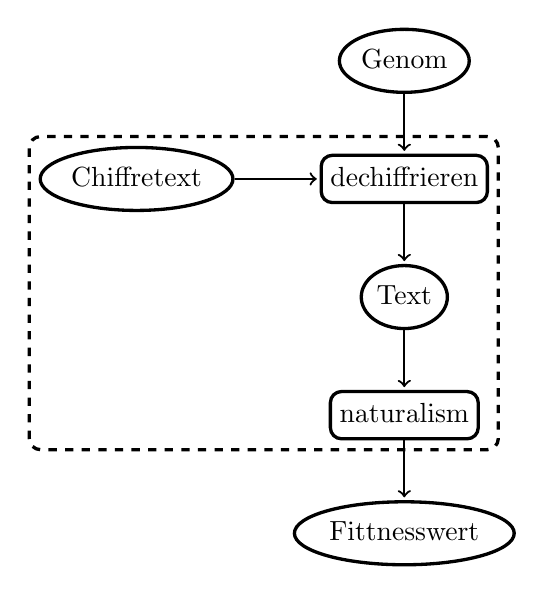
\begin{tikzpicture} [ node distance =1.5cm
								, text depth = .25ex
								, text height =1.5ex
								, value/.style={ellipse, minimum height=.8cm, inner sep=1pt, very thick, draw}
								, funktion/.style={rectangle, rounded corners, minimum size=6mm, very thick, draw}
								, pfeilspitze/.style ={draw, thick, shorten >=1pt, arrows= ->}
								]
	\node (Genom) 			[value] {Genom};
	\node (dechiffrieren) 	[funktion, below of = Genom] {dechiffrieren};
	\node (Chiffretext) 		[value, node distance =3.4cm, left of = dechiffrieren] {Chiffretext};
	\node (Klartext) 			[value, below of = dechiffrieren] {Text};
	\node (naturalism) 		[funktion, below of = Klartext] {naturalism};
	\node (Fittness) 			[value, below of = naturalism] {Fittnesswert};

	\node [funktion, dashed, draw, fit=(Chiffretext) (dechiffrieren) (Klartext) (naturalism) ]{};

	
	\draw [pfeilspitze] (Chiffretext) -- (dechiffrieren);
	\draw [pfeilspitze] (Genom) -- (dechiffrieren);
	\draw [pfeilspitze] (dechiffrieren) -- (Klartext);
	\draw [pfeilspitze] (Klartext) -- (naturalism);
	\draw [pfeilspitze] (naturalism) -- (Fittness);

\end{tikzpicture}